\chapter{Implementation}
The implementation of each part of the system was made with application of Test Driven Development which guarantees full test coverage for the code. Used testing framework is \textit{mocha} \url{https://mochajs.org/}. For creation of doublers (mocks, stubs and spies) for object and method was used \textit{sinon.js }\url{http://sinonjs.org/}. 
The implementation of the system was made with respect to principles of agile architecture \cite{Dooley}\cite{MartinASD} :
\begin{itemize}
	\item Closing - Encapsulate things in your design that are likely to change.
	\item Code to an Interface - rather then to an implementation. 
	\item Do not repeat yourself - Avoid duplicate code.
	\item The Single-Responsibility Principle - A class should have only one reason to change
	\item The Open/Closed Principle - Software entities (classes, modules, functions, etc.) should be open for extension but closed for modification
	\item The Liskov Substitution Principle - Subtypes must be substitutable for their base types.
	\item The Dependency-Inversion Principle - A) High-level modules should not depend on low-level modules. 
	Both should depend on abstractions. 
	B) Abstractions should not depend upon details. 
	Details should depend upon abstractions.
	\item The Interface Segregation Principle - Clients should not be forced to depend on methods they do not use.
	\item Principles of Least Knowledge - Talk to your immediate friends. 
	\item Principle of Loose Coupling - object that interact should be loosely coupled with well-defined intefaces.
\end{itemize}
If violation of any of this principles will take place it will be stated explicitly.

For description of data structures processed by the system we will use following module (Listing: \ref{demo}) which implements stack with asynchronous methods (respond time for each method is 10 milliseconds). Usage of setTimeout() method guaranties its asynchronism while the fact that timeframe for response hardcoded into scraping scripts guarantees that this method is valid for usage as a proof of concept in current research topic.
\lstinputlisting[
language=Javascript, numbers=left, stepnumber=5, firstnumber=1, breaklines=true, 
basicstyle=\footnotesize,
numberstyle=\tiny,
caption={stack.js},
captionpos=b,
label=demo
]
{code/demo/stack.js.txt}
The Test Sheet for test coverage of this module looks as following (Figure: \ref{fig:demoTS}). Note that in invocation line E there are both types of comparison.
\begin{figure}
\centering
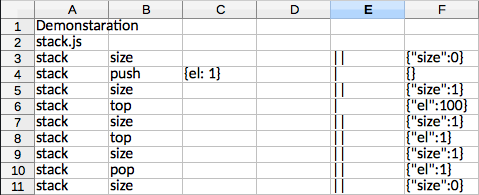
\includegraphics[scale=0.7]{grafiken/demoTS}
\caption{Test Sheet coverage for stack.js}
\label{fig:demoTS}
\end{figure}



\section{Read Stream}

This part of the system is an implementation of combining streams pattern. From the internal view it consists of two streams. First stream performs recursive search for files in a provided directory and returns array with absolute paths to them. Second stream reads content of files with \textit{xlsx} module \url{https://www.npmjs.com/package/xlsx} and meta data of the file using embedded node.js module \textit{fs} and pushes it to the up stream.

\lstinputlisting[
language=Javascript, numbers=left, stepnumber=5, firstnumber=1, breaklines=true, 
basicstyle=\footnotesize,
numberstyle=\tiny,
caption={stack.js},
captionpos=b,
label=demo
]
{code/lib/stream/readStream.js.txt}

\textbf{The function getFilesStream} creates readable stream for reading content of directory including nested directories and returns it. 
\textbf{The variable getDataStream} defined by stream in a object mode. For every file path it accepts from the down stream  checks its extensions if its .xlsx then it reads it and obtains first sheet from the book, and reads meta data of the file and pushes it to the up stream.
This two streams are piped in to combined stream using module \textit{multipipe} \url{https://www.npmjs.com/package/multipipe} and returned by the function exported by this module.
In other words, this module exports function which accepts path to the directory and returns array of deferred values each of which is a javascript object with following structure: \{ fileName: file, meta: meta, sheet: sheet \}.


%\paragraph{Correspondence to design principles:}
%\begin{itemize}
%	\item Closing - stream is closed over file extension, schema\_maker - object structure returned by 	\textit{xlsx} library;
%	\item Code to Interface - stream obtains and returns values via standard stream interface, call to file system made via standard nodeJS File System stream interface;
%	\item Do not Repeat Yourself - no code duplication;
%	\item Single Responsibility Principle - can be changed only due to the change of input type;
%	\item Open Close Principle - new pipes can be added in a single place;
%	\item Liscov Substitution Principle - no inherited objects used;
%	\item Interface Segregation Principle - no dependency on redundant methods;
%	\item Dependency Inversion Principle - higher level module index.js does not depend on current library
%	\item Least Knowledge Principle - communication to interfaces and invocation of used library;
%	\item Loose Coupling Principle - standard interfaces;
%\end{itemize}
%
%\textbf{Design principles implication:}
%\begin{itemize}
%\item  S. - Single Responsibility Principle - can be changed only due to the change of input type
%\item  O. - Open Close Principle - new pipes can be added in a single place
%\item  L. - Liscov Substitution Principle - no inheritance
%\item  I. - Interface Segregation Principle - Stream interface / File System interface
%\item  D. - Dependency Inversion Principle - Higgher level module index.js does not depend on current library
%
%Writer structure:\\


\section{Transform Stream}

\section{Write Stream}

\section{Compare and Write module}